\documentclass[cn,hazy,black,11pt,normal]{elegantnote}
\title{最优化算法实验报告}

\author{陈文轩}
\usepackage{array}
\usepackage{amsfonts}
\usepackage{float}
\usepackage{mathtools}


\newcommand*{\dif}{\mathop{}\!\mathrm{d}}
\DeclareMathOperator*{\st}{s.t.\,\,}
\DeclareMathOperator*{\argmin}{arg\,min}
\DeclareMathOperator*{\argmax}{arg\,max}
\DeclareMathOperator*{\sgn}{sgn}
\date{\today}

\begin{document}

\maketitle
    \section{基本模型与优化目标}

        \subsection{任务与目标}

            \begin{itemize}
                \item 任务:对二分类数据$\{(a_i,b_i)\}_{i=1}^m$,其中$b_i\in\{-1,+1\}$,学习稀疏权重向量$x\in\mathbb{R}^n$。
                \item 目标函数:\[\min_x\ell(x)=\dfrac1m\sum_{i=1}^m \log\left(1+\exp\left(-b_i a_i^{\top}x\right)\right)+\lambda\|x\|_2^2+\mu\|x\|_1,\]
                    \begin{itemize}
                        \item 第一项是逻辑回归损失函数。
                        \item 第二项$\lambda\|x\|_2^2$提供$L^2$正则化,帮助数值稳定并减少共线性。
                        \item 第三项$\mu\|x\|_1$提供$L^1$正则化,促进稀疏性。
                        \item $\ell(x)$是一个凸函数。
                    \end{itemize}
            \end{itemize}
    
        \subsection{ADMM 变量拆分与增广拉格朗日函数}

            为了处理非光滑的$L^1$项,引入辅助变量$z$,并添加约束$x=z$:\[\min_{x,z}\dfrac1m\sum_{i=1}^m \log\left(1+\exp\left(-b_i a_i^{\top}x\right)\right)+\lambda\|x\|_2^2+\mu\|z\|_1,\quad\st x=z,\]

            增广拉格朗日函数为:\[\mathcal{L}_{\rho}(x,z,y)=\dfrac1m\sum_{i=1}^m \log\left(1+\exp\left(-b_i a_i^{\top}x\right)\right)+\lambda\|x\|_2^2+\mu\|z\|_1+\dfrac{\rho}2\|x-z\|_2^2+y^{\top}(x-z),\]

            令$v_k=z_k-\dfrac{y_k}{\rho}$即可得到ADMM的各个子问题:

            \begin{enumerate}
                \item $x\,$-子问题:\[x_{k+1}=\argmin_x\left(\dfrac1m\sum_{i=1}^m \log\left(1+\exp\left(-b_i a_i^{\top}x\right)\right)+\lambda\|x\|_2^2+\dfrac{\rho}2\|x-v_k\|^2\right)\]
                \item $z\,$-子问题:\[z_{k+1}=\argmin_z\left(\mu\|z\|_1+\dfrac{\rho}2\|v_{k+1}-z\|^2\right)\]
                \item 对偶更新:\[y_{k+1}=y_k+\rho(x_{k+1}-z_{k+1})\]
            \end{enumerate}

        \subsection{子问题求解}

            \subsubsection{$x\,$-子问题}

                $x$-子问题是一个光滑的凸优化问题,可以使用牛顿法等方法求解:

                \begin{itemize}
                    \item 梯度:\[\nabla f(x)=\dfrac1mA^{\top}\left(\sigma(-b\odot(Ax))-b\right)+2\lambda x+\rho(x-v_k),\]其中$\sigma(t)=\dfrac1{1+e^{-t}}$。
                    \item Hessian矩阵:\[H\coloneqq\nabla^2 f(x)=\dfrac1mA^{\top}DA+(2\lambda+\rho)I,D_{ij}=\delta_{ij}\sigma(-b_i a_i^{\top}x)(1-\sigma(-b_i a_i^{\top}x))\]
                    \item 方向:$p_k=-H^{-1}\nabla f(x)$,若出现奇异或方向上升,则退化为负梯度步。
                    \item 步长:Armijo条件$f(x+tp_k)\leq f(x)+c_1 t\nabla f^{\top}p_k$,程序中取$c_1=0.01,\beta=0.5$。
                    \item 终止条件:$\|tp_k\|_2<10^{-7}$或迭代次数满\texttt{max\_newton\_iter}。
                \end{itemize}

                上述细节完全对应\texttt{x\_update\_objective\_and\_grad\_hess}与\texttt{solve\_x\_subproblem}函数。

            \subsubsection{$z\,$-子问题}

                $z\,$-子问题有解析解\[z_{k+1}=S_{\frac{\mu}{\rho}}\left(x_{k+1}+\dfrac{y_k}{\rho}\right),\]

                其中软阈值算子定义为\[S_{\kappa}(u)=\sgn(u)\max\{|u|-\kappa,0\}\]

                实现见\texttt{soft\_threshold}函数。

        \subsection{收敛判据}

            原始残差$r_k^{\text{pri}}=\|x_k-z_k\|_2$,对偶残差$r_k^{\text{dual}}=\rho\|z_k-z_{k-1}\|_2$,当$\max\{r_k^{\text{pri}},r_k^{\text{dual}}\}<\text{tol\_abs}=10^{-6}$时认为收敛。



    \section{实验结果}

        $\lambda=\dfrac1{2m},\mu=0.01$时ADMM两个最优条件与迭代步数的关系图以及误差与迭代步数的关系图如下所示:

        \begin{figure}[H]
            \centering
            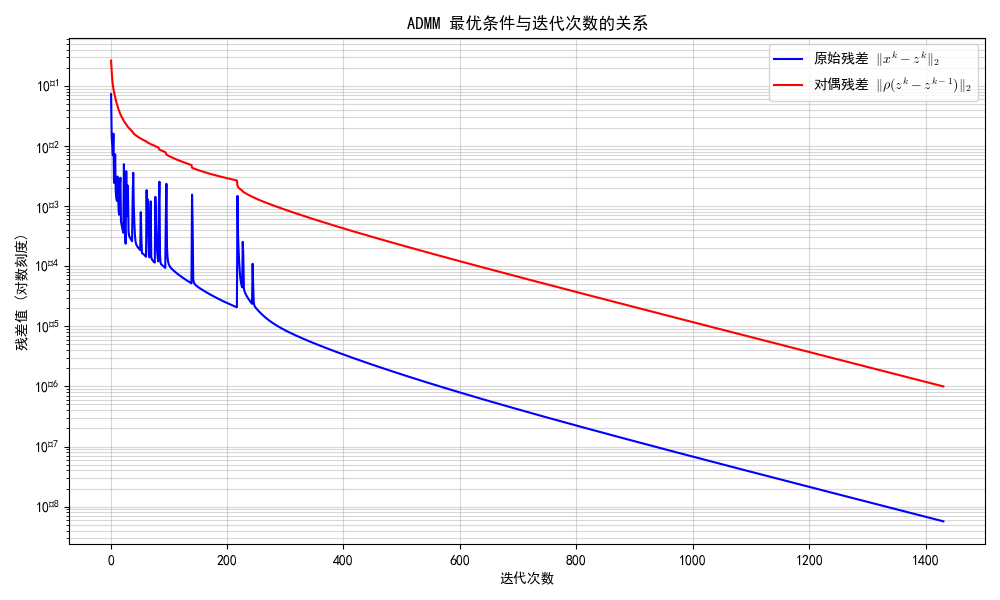
\includegraphics[width=0.98\textwidth]{image/admm_residuals_cn}
            \caption{ADMM原始残差与对偶残差}
            \label{fig:admm_residuals}
        \end{figure}

        \begin{figure}[H]
            \centering
            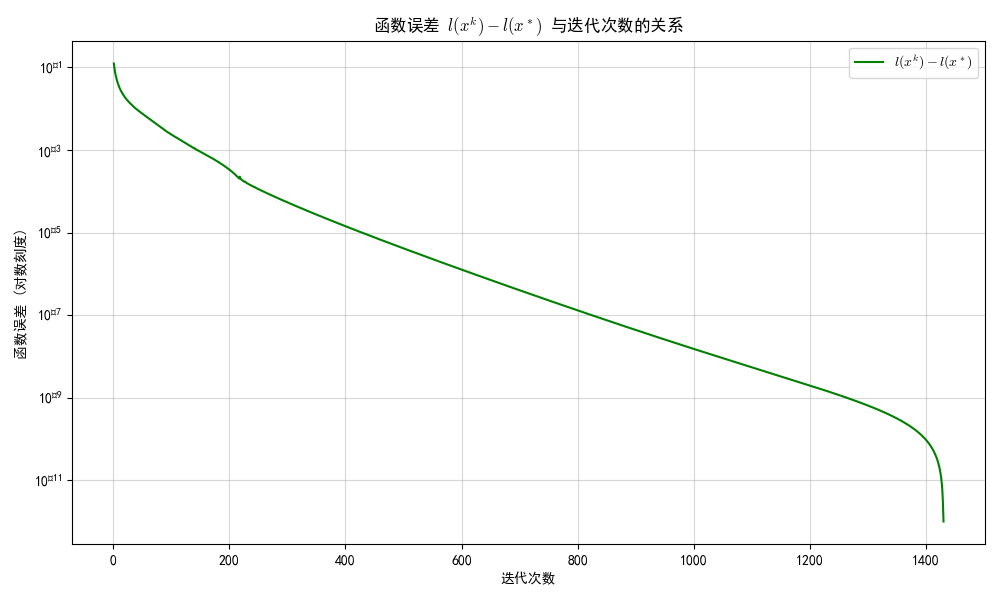
\includegraphics[width=0.98\textwidth]{image/function_error_cn}
            \caption{ADMM目标函数误差}
            \label{fig:function_error}
        \end{figure}

        迭代步数,稀疏度与$\mu$的关系如下表所示:

        \begin{table}[H]
            \centering
            \begin{tabular}{|c|c|c|c|}
                \hline
                $\mu$ & 迭代步数 & 稀疏度 & 非零元数量 \\
                \hline
                $0.001$ & $4570$ & $0.6829$ & $39$ \\
                $0.01$ & $1430$ & $0.8862$ & $14$ \\
                $0.05$ & $645$ & $0.9675$ & $4$ \\
                $0.1$ & $204$ & $0.9675$ & $4$ \\
                \hline
            \end{tabular}
            \caption{ADMM迭代步数与稀疏度}
            \label{tab:admm_iterations}
        \end{table}

        可以发现,随着$\mu$的增大,迭代步数减少,稀疏度增加,非零元数量减少。$\mu=0.05$时,模型非常稀疏,仅有4个非零元。

    \section{参数选取}

        \begin{table}[H]
            \centering
            \scalebox{0.75}{
            \begin{tabular}{|c|c|c|c|}
                \hline
                参数 & 作用 & 默认值 & 说明 \\
                \hline
                $\lambda$ & $L^2$正则化系数 & $\tfrac1{2m}$ & 控制模型复杂度,防止过拟合 \\
                $\mu$ & $L^1$正则化系数 & $0.001,0.01,0.05$ & 促进稀疏性,选择特征 \\
                $\rho$ & ADMM增广拉格朗日参数 & $1$ & 控制原始和对偶残差的平衡 \\
                \texttt{max\_admm\_iter} & ADMM最大迭代次数 & $10000$ & 过大仅保证极端情况。 \\
                \texttt{max\_newton\_iter} & 牛顿法最大迭代次数 & $20$ & 若单次步长极小/收敛慢,可增大;但超50回报递减 \\
                \texttt{tol\_abs} & 收敛判据绝对容忍度 & $10^{-6}$ & 原始和对偶残差均小于此值时认为收敛 \\
                \texttt{bt\_c1,bt\_beta} & Armijo条件参数 & $0.01,0.5$ & 通常保持默认即可;若目标函数震荡可减小\texttt{bt\_beta} \\
                \hline
            \end{tabular}}
            \caption{ADMM参数选取}
            \label{tab:params}
        \end{table}
\end{document}